%
% Annual Cognitive Science Conference
% Sample LaTeX Paper -- Proceedings Format
%

% Original : Ashwin Ram (ashwin@cc.gatech.edu)       04/01/1994
% Modified : Johanna Moore (jmoore@cs.pitt.edu)      03/17/1995
% Modified : David Noelle (noelle@ucsd.edu)          03/15/1996
% Modified : Pat Langley (langley@cs.stanford.edu)   01/26/1997
% Latex2e corrections by Ramin Charles Nakisa        01/28/1997
% Modified : Tina Eliassi-Rad (eliassi@cs.wisc.edu)  01/31/1998
% Modified : Trisha Yannuzzi (trisha@ircs.upenn.edu) 12/28/1999 (in process)
% Modified : Mary Ellen Foster (M.E.Foster@ed.ac.uk) 12/11/2000
% Modified : Ken Forbus                              01/23/2004
% Modified : Eli M. Silk (esilk@pitt.edu)            05/24/2005
% Modified : Niels Taatgen (taatgen@cmu.edu)         10/24/2006
% Modified : David Noelle (dnoelle@ucmerced.edu)     11/19/2014
% Modified : Roger Levy (rplevy@mit.edu)     12/31/2018



%% Change "letterpaper" in the following line to "a4paper" if you must.

\documentclass[10pt,letterpaper]{article}

\usepackage{cogsci}

\cogscifinalcopy % Uncomment this line for the final submission

\usepackage{amsmath}
\usepackage[c]{esvect}
\usepackage{pslatex}
\usepackage{apacite}
\usepackage{enumitem}
\setlist{noitemsep,topsep=0pt,parsep=0pt,partopsep=0pt,leftmargin=*}
\usepackage{graphicx}
\usepackage{dblfloatfix}
\usepackage{float} % Roger Levy added this and changed figure/table
                   % placement to [H] for conformity to Word template,
                   % though floating tables and figures to top is
                   % still generally recommended!

%\usepackage[none]{hyphenat} % Sometimes it can be useful to turn off
%hyphenation for purposes such as spell checking of the resulting
%PDF.  Uncomment this block to turn off hyphenation.


%\setlength\titlebox{6.5cm}
% You can expand the titlebox if you need extra space
% to show all the authors. Please do not make the titlebox
% smaller than 4.5cm (the original size).
%%If you do, we reserve the right to require you to change it back in
%%the camera-ready version, which could interfere with the timely
%%appearance of your paper in the Proceedings.


\title{How do blind people know that blue is cold? \\ Distributional semantics encode color-adjective associations.}

\author{{\large \bf Jeroen van Paridon (vanparidon@wisc.edu)} \\
  %Department of Psychology, University of Wisconsin-Madison \\
  %1202 W. Johnson Street, Madison, WI 53706 USA
  \AND {\large \bf Qiawen Liu (qliu295@wisc.edu)} \\
  %Department of Psychology, University of Wisconsin-Madison \\
  %1202 W. Johnson Street, Madison, WI 53706 USA
  \AND {\large \bf Gary Lupyan (lupyan@wisc.edu)} \\
  \\
  Department of Psychology, University of Wisconsin-Madison \\
  1202 W. Johnson Street, Madison, WI 53706 USA}

\begin{document}

\maketitle

\begin{abstract}
Certain colors are strongly associated with certain adjectives (e.g. red is hot, blue is cold). Some of these associations are grounded in visual experiences like seeing hot embers glow red. Surprisingly, many congenitally blind people show similar color associations, despite lacking all visual experience of color. Presumably, they learn these associations via language. Can we detect these associations in the statistics of language? And if so, what form do they take? We apply a projection method to word embeddings trained on corpora of spoken and written text to identify color-adjective associations as they are represented in language. We show that these projections are predictive of color-adjective ratings collected from blind and sighted people, and that the effect size depends on the training corpus. Finally, we examine how color-adjective associations might be represented in language by training word embeddings on corpora from which various sources of color-semantic information are removed.

\textbf{Keywords:}
distributional semantics; language and thought; word associations
\end{abstract}

\section{Introduction}
Much of what we know about the world we learn by perceiving and interacting with it, and consequently we often talk about knowledge as if it can only be acquired through personal experience. This has sometimes led to the presumption that people who lack certain experiences (e.g. because they are blind or deaf) do not understand the nature of these experiences. It was long thought, for instance, that blind people could not understand the concept of color \cite<see e.g.,>{hume1740treatise,locke1690essay}. Evidence from behavioral studies, however, suggests that blind participants can in fact distinguish between cool and warm colors \cite{shepard1992representation} and that some are able to rate color similarities with enough accuracy that multidimensional scaling of the pairwise similarities yields an arrangement that resembles the color wheel \cite{marmor1978age,saysani2018colour}. Most recently, \citeA{saysani2021seeing} collected semantic differential ratings for color words from both blind and sighted individuals and used multidimensional scaling to demonstrate that there is considerable variability between blind individuals and that some, but not all, blind participants generate semantic differentials that are highly similar to the ones generated by sighted people. Since blind participants have no means of directly perceiving color associations, it perhaps seems obvious that they learn color semantics from language. \emph{How} color semantics are represented in spoken and written language--and to what extent language, rather than visual perception, aligns color semantics between individuals--is, however, not obvious. Are color semantics conveyed explicitly, e.g. through generic statements? Are they conveyed through simple co-occurrences, when a color word occurs adjacent to another word? Or are color semantics encoded in more complex semantic structures--a web of associations that we can derive color semantics from?

We conduct four experiments to further explore these questions: In Experiment 1 we reanalyze data collected by \citeA{saysani2021seeing} using word embeddings (a class of distributional semantics model) to get a quantitative measure of the relationship between participants' color-adjective association ratings and the color semantics represented in language. In Experiment 2 we replicate our findings from Experiment 1 in a sighted sample of American English speakers and further ask whether participants think their own color associations differ from those of others. In Experiment 3 we replicate our findings in yet another, larger, sighted sample, and also explore whether more exposure to certain kinds of language causes participants' color-adjective associations to be more aligned. In Experiment 4, we test several hypothesized origins of color-adjective associations in word embeddings by selectively removing them from the corpus on which the embeddings are trained.

\section{Experiment 1: Reanalysis of \citeauthor{saysani2021seeing}}
\subsection{Word embedding projections}
Using word embeddings, we draw an axis from one end of a semantic dimension (e.g. \emph{hot}) to the other end (e.g. \emph{cold}) by subtracting the word vector for one of the two adjectives from the word vector for the other adjective, and then project the word embedding for each color onto that axis by computing the cosine similarity between the color word vector and the axis vector. The projection for e.g. the color blue on the dimension cold-hot is then given by $\cos{(\vv{\text{hot}} - \vv{\text{cold}}, \vv{\text{blue}})}$ (see \citeNP{grand2018semantic} for a discussion of this projection method, but note that the method we use here differs slightly in that we normalize the semantic axis by its L2-norm before computing the inner product, which is equivalent to taking the cosine similarity). This provides us with a relative measure of word similarity, taken along the semantic dimension's axis, that we can use to predict human ratings of color associations.

Word embeddings are trained on large text corpora, and as such the semantic information they capture tends to reflect the contents of the corpus they are trained on. Using the projection method, we computed color associations in 300-dimensional embeddings trained on several different text corpora: embeddings pretrained on Common Crawl and Wikipedia using the \emph{fastText} implementation of the continuous bag of words (CBOW) model \cite{grave2018learning}, embeddings pretrained on the OpenSubtitles corpus using the \emph{fastText} implementation of the skipgram model  \cite{van2020subs2vec}, and embeddings trained on the subcorpora of the Corpus of Contemporary American English (COCA; subcorpora are fiction, news, academic texts, spoken texts, and magazine articles) using the \emph{fastText} implementation of the skipgram algorithm \cite<\emph{fastText} uses subword information to improve embeddings, for details of the CBOW and skipgram implementations see>{bojanowski2017enriching}.

\section{Method}

\subsection{Participants}
\citeauthor{saysani2021seeing} recruited 32 participants, all native speakers of English, 20 of whom had normal, trichromatic vision (mean age = 29, range = 21--35). The remaining 12 were congenitally blind with no residual experience of vision (mean age = 39.6, range = 18--69).
\subsection{Design and procedure}
Participants were asked to rate each of nine color terms (red, orange, yellow, green, blue, brown, purple, black, and white) on 17 semantic dimensions, each defined by two antonyms placed at the poles of a seven-point Likert scale (happy–sad, calm–angry, submissive–aggressive, relaxed–tense, exciting–dull, selfless–jealous, active–passive, like–dislike, alive–dead, fast–slow, new–old, unripe–ripe, soft–hard, light–heavy, fresh–stale, clean–dirty, and cold–hot). See Figure \ref{color_ratings} for lowest- and highest-rated colors in each dimension.
\section{Results}
The main finding reported by \citeA{saysani2021seeing} was that multidimensional scaling solutions were more variable between blind participants than between sighted participants. Comparing intraclass correlations (ICC) for the blind (.35, 95\% CI [.29, .42]) and the sighted (.49, 95\% CI [.43, .55]) groups also suggests the blind participants are more variable than the sighted participants and computing ICCs for repeated sub-samples from the sighted group suggests this difference is not simply due to the smaller number of blind participants. However, slightly higher between-participant variability does not mean that there is no common variance in individual blind participants' scores that can be predicted from a common measure.

\begin{figure}[ht!]
\begin{center}
\fbox{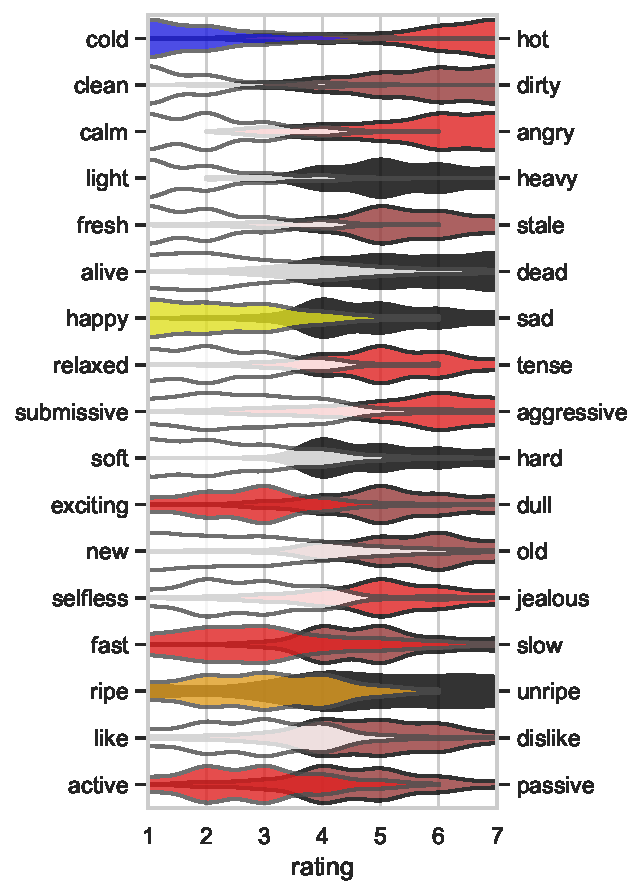
\includegraphics[width=\columnwidth]{figures/color_ratings.pdf}}
\caption{Distribution of participants' color-adjective association ratings for the lowest- and highest-rated color on each dimension. Dimensions are plotted in order of mean color rating variance (with the most differentiated dimension, ``cold-hot'' at the top of the figure). This figure combines participant ratings from Experiments 1-3.}
\label{color_ratings}
\end{center}
\end{figure}

Using a Bayesian linear mixed-effects model with weakly regularizing priors \cite{yarkoni2016bambi}, we regressed word embedding projections onto participants' color-adjective association ratings, while adjusting for dimension word frequency and dimension word concreteness (these are included as nuisance predictors; we are not particularly interested in their effects, but if they \emph{are} affecting ratings we want to account for that source of variability). The model accounts for random variability by including participant-, color-, and dimension-level random intercepts but also participant-level random slopes for embedding projections, dimension word frequency, and dimension word concreteness.

Color-adjective ratings (e.g., placing yellow closer to ripe than unripe) were predicted by word embedding projections, with a standardized effect size of .68 (95\% CI [.59, .77]) for sighted participants and .46 (95\% CI [.34, .57]) for blind participants when using the COCA-fiction based embeddings, meaning a shift of one standard deviation in embedding projections predicted a shift of .68 and .46 standard deviations, respectively, in color-adjective ratings from sighted and blind participants. Effect sizes were smaller for the other training corpora, with COCA-spoken performing worst. The COCA-fiction effect sizes are relatively large, but we cannot tell from just the size of the effect whether it is a broad effect across dimensions and colors, or if it is driven by a small number of highly salient color-adjective pairs (e.g. \emph{unripe} and \emph{green}). We can, however, adjust for these highly salient pairs by including as a predictor how often a given color was provided as response by people being cued with an adjective in the Small World of Words word association corpus \cite<SWOW;>{de2019small}. For instance, given the cue ``unripe'', 18\% of people responded with ``green''. We then compute SWOW differential scores by subtracting the number of ``green'' responses to the cue ``ripe'' from the number of ``green'' responses to ``unripe''. Participants in the SWOW study provided three responses to each cue word; we included all three responses in our SWOW differential calculation. SWOW and embedding projections are only very weakly correlated (correlations range from .09 to .12, depending on embedding training corpus) suggesting that these measures describe different sources of semantic association.

Color-adjective ratings were predicted by both SWOW differential scores and by word embedding projections, however adjusting for SWOW differential caused only a minor reduction in the effect sizes of the word embedding projections: SWOW differential scores have an estimated standardized effect size of .25 (95\% CI [.29, .21]); word embedding projections have an estimated standardized effect size of .58 (95\% CI [.66, .50]) in sighted participants and .37 (95\% CI [.48, .26]) in blind participants when trained on COCA-fiction (see Figure \ref{original} for all effect size estimates).

\begin{figure}[ht!]
\begin{center}
\fbox{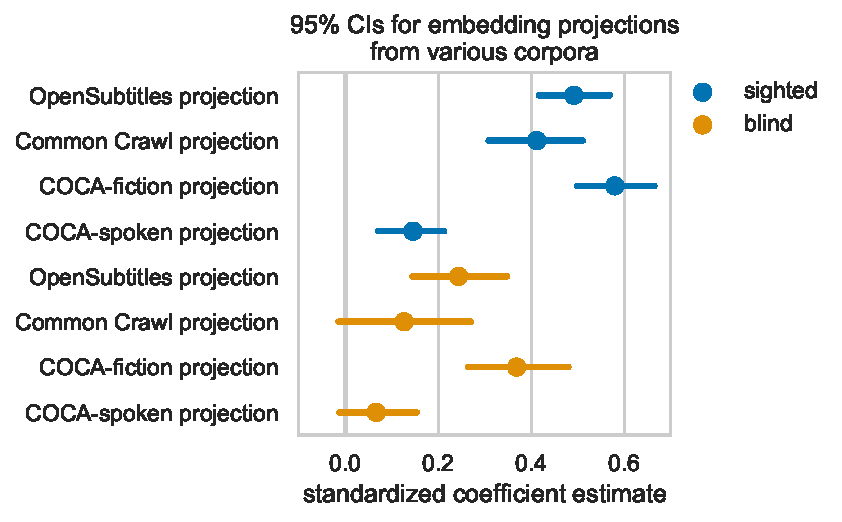
\includegraphics[width=\columnwidth]{figures/original_forest_new.pdf}}
\caption{Estimated effects of word embedding projections from various corpora in predicting sighted and blind participants' color-adjective association ratings from Experiment 1.}
\label{original}
\end{center}
\end{figure}

\section{Discussion}
Color-adjective associations in language may arise from our visual perception of the world around us, but they appear to be predictive for both blind and sighted participants' ratings of color-adjective associations. This suggests that even though blind participants are more variable in their color-adjective association ratings, this information is contained, to some extent, in the statistics of language, allowing blind people to align their color semantics with those of sighted people. The alignment is not perfect, of course, but consider that in the absence of a shared language, no such alignment would be possible at all.

\subsection{Differences between embedding training corpora}
Each of the corpora we used yielded color associations that were predictive of the human ratings of color associations, but the corpus that yielded the most predictive associations (i.e. the largest effect size) was the fiction subcorpus of the Corpus of Contemporary American English (COCA-fiction). This is unrelated to the relative sizes of the training corpora: We controlled the sizes of the different COCA-subcorpora specifically to allow for direct comparisons between different registers of English (and fiction clearly outperformed e.g. spoken English here). Moreover, the OpenSubtitles corpus is about 50\% larger than the COCA-subcorpora and the Common Crawl corpus is about an order of magnitude larger, yet neither of these corpora produced embeddings as predictive of color-adjective associations as the COCA-fiction embeddings.

There are a number of reasons why fiction specifically, would render a high quality representation of color associations: The fiction subcorpus has a wide-ranging semantic scope and contains long, coherent sentences. It is therefore relatively high in quality compared to e.g. the spoken subcorpus, which largely consists of news shows and talk radio interviews and is therefore more limited in semantic scope and contains many short or disjointed sentences. However, what is likely most important is that fiction contains many idiomatic expressions that convey--or are even the primary source of--color associations, such as stating someone is turning blue (when they are cold), green (with jealousy), or red (with anger or embarrassment). These idioms are less common or even absent in news and academic texts, and may be less consistently used in spoken text.

\subsection{Between-participant variability}
That we are able to use word embeddings to predict people's color-adjective ratings means that these ratings are, to some extent, similar. Not all variability in participant ratings is predicted by word embeddings however, and intraclass correlations between participants suggest that there is a considerable amount of variability between participants. Some of this variability may be due to sampling error, but another source could be that participants' color semantics are idiosyncratic, shaped by experiences unique to each individual. For example, you you might think yellow is associated with calmness because the yoga studio you go to has yellow walls.


\section{Experiment 2: Replication of sighted results}
To test whether participants perceived their own color-adjective associations as idiosyncratic, we conducted a replication of Experiment 1 with sighted participants, whom we asked to provide not only color-adjective association ratings for themselves (\emph{self-ratings}), but also their expectation of color-adjective association ratings other participants would provide (\emph{other-ratings}).
\section{Method}
\subsection{Participants}
We recruited 30 undergraduate psychology students from the student participant pool at the University of Wisconsin-Madison.
\subsection{Design and procedure}
Stimuli and procedure were identical to those used in Experiment 1, with two exceptions:
\begin{enumerate}
\item The experiment was carried out online rather than in person.
\item We asked participants to provide not only their own color-adjective association ratings, but also the color-adjective associations they expected others would provide.
\end{enumerate}

\section{Results}
Using the model structure described in Experiment 1, with the addition of a binary variable describing whether a rating is a self- or an other-rating (and interactions between that variable and the various other variables), we again regress word embedding projections and SWOW differential scores onto participants' color-adjective association ratings.

Participants' self- and other-ratings were almost perfectly correlated (Pearson r = .98). Bayesian linear mixed effects modeling showed no difference in self- versus other-ratings (mean estimated effect size .00, 95\% CI [-.03, .04]) and embedding projections nor SWOW differential scores were equally predictive of self- and other-ratings (mean estimated interaction for embedding projections and self- vs. other-ratings .01, 95\% CI [-.01, .03], mean estimated interaction for SWOW differential scores and self- vs. other-ratings .00, 95\% CI [-.02, .02]), for effect sizes in self- and other-ratings see Figure \ref{self_other}.

\begin{figure}[ht!]
\begin{center}
\fbox{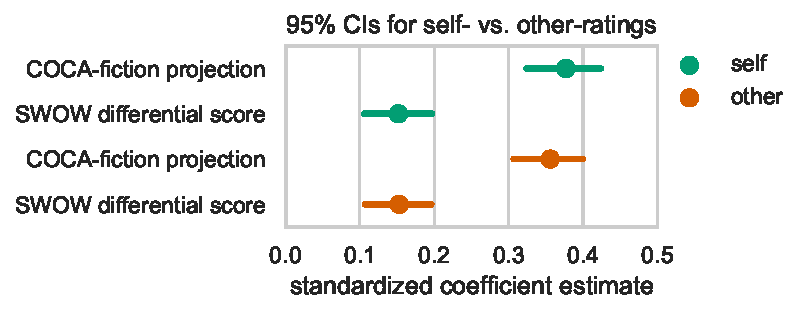
\includegraphics[width=\columnwidth]{figures/self_other_forest_new.pdf}}
\caption{Estimated effects of word embedding projections and SWOW differential scores in predicting sighted participants' color-adjective self-ratings and other-ratings from Experiment 2.}
\label{self_other}
\end{center}
\end{figure}

\section{Discussion}
While some color-adjective associations may indeed be idiosyncratic, participants certainly do not perceive their own associations as differing from others'.

\section{Experiment 3: Do people who read more have ratings more similar to the fiction corpus?}
\section{Method}
\subsection{Participants}
We recruited 100 undergraduate psychology students from the student participant pool at the University of Wisconsin-Madison.
\subsection{Design and procedure}
Stimuli and procedure were identical to those used in Experiment 1, with two exceptions:
\begin{enumerate}
\item The experiment was carried out online rather than in person.
\item We asked participants to fill out a survey meant to assess their exposure to fiction texts, including how many hours per week they spend reading fiction and nonfiction text and a series of questions meant to gauge reading motivation. Participants also completed the Author Recognition Test \cite<ART;>{acheson2008new}. The ART is meant to assess a participant's familiarity with prominent authors and is a well-validated proxy of print exposure.
\end{enumerate}

\section{Results}
We analyzed this experiment using the model described in Experiment 1, with added predictors for the reading measures and their interaction with the word embedding projections from the COCA-fiction corpus.
None of the reading measures interact with the word embeddings projections in predicting color-adjective association ratings (see Figure \ref{reading_measures} for estimated effect sizes).

The intraclass correlation of participants' self-ratings was lower in this experiment (.27, 95\% CI [.23, .32]) than in than in Experiment 1. One possible reason for this increased variability despite the larger sample size is that participants in Experiment 1 participated in a lab setting, whereas the present experiment had to be conducted online. This increase in between-participant variability could explain why the effect size for the COCA-fiction projections is somewhat smaller in the present experiment than in Experiment 1.

\begin{figure}[ht!]
\begin{center}
\fbox{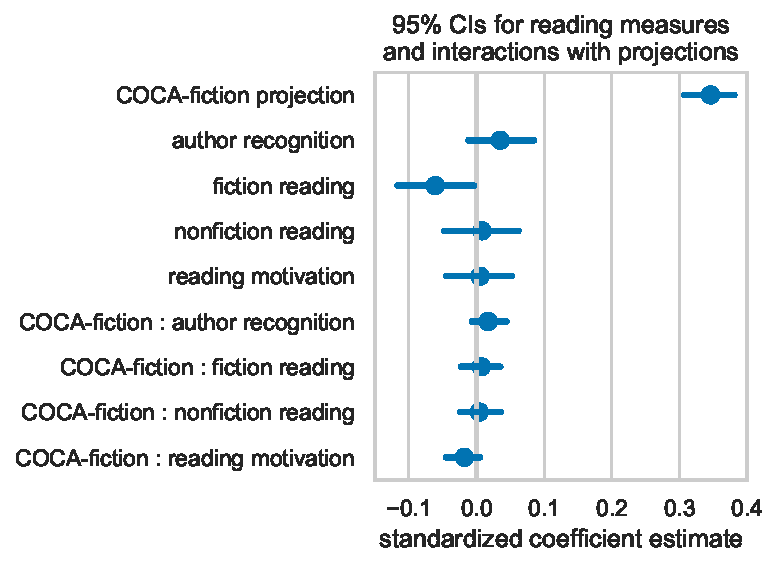
\includegraphics[width=\columnwidth]{figures/reading_measures_forest_new.pdf}}
\caption{Estimated effects of word embedding projections, various reading measures, and the interactions between projections and reading measures in predicting sighted participants' color-adjective association ratings from Experiment 3. The predictiveness of fiction-derived word embedding projections does not appear to be higher for participants with more reading exposure.}
\label{reading_measures}
\end{center}
\end{figure}

\section{Discussion}
Given the predictive power of the COCA-fiction word embedding projections (relative to those based on spoken text or Wikipedia/Common Crawl), it is surprising that reading more fiction does not cause participants to be more aligned with the word embedding projections. However, it is possible that since our participants are all undergraduate students at a large research university, their shared linguistic and cultural background (reading the same books in school, watching the same TV shows growing up, using the same social media) could mean they are already strongly semantically aligned, essentially creating a ceiling effect that obscures any alignment due to additional exposure to written fiction.

\subsection{Where do the embeddings ``learn'' their color semantics?}
One potential way of finding the source of these color associations (in the word embeddings, at least) is to try to modify the training corpus in such a way that the associations disappear from the embeddings (and the projected associations are no longer predictive of human ratings). If we can identify the sentences in the training corpus that give rise to the color associations, can these sentences tell us whether (and how) humans learn color associations from language?

\section{Experiment 4: Identifying sources of color-adjective associations in embeddings}
Identifying the sentences that are most informative for color associations in a training corpus is not a trivial problem: there is a computational cost to training word embeddings, so performing an exhaustive search is not feasible. Nevertheless, we can start by testing several "naive" hypotheses of what is responsible for the color-adjective associations we find in the word embedding models: 
\begin{enumerate}[label=(\alph*)]
\item \emph{First-order} co-occurrences: the occurrence of a color word and a semantic dimension word in the same sentence (e.g. "the fire was \emph{red hot}"; color associations in these sentences can be explicit, but often are not).
\item \emph{Second-order} co-occurrences: the occurrence of color words and semantic dimension words in similar contexts (i.e. color words and semantic dimension words may not co-occur, but the share words that they co-occur with, e.g. "Southern cooking uses \emph{green} tomatoes" and "Southern cooking uses \emph{unripe} tomatoes").
\item Co-occurrences between color words and words in the same semantic neighborhood as semantic dimension words. For example in "The forest was \emph{white} with \emph{snow}", \emph{snow} is in the same semantic neighborhood as \emph{cold}, which might lead to an association between \emph{white} and \emph{cold}). We can identify semantic neighborhood words using cosine similarity between word embeddings.
\item Mediation by psychologically salient words. It is conceivable that some color-adjective associations may be driven by mediation by specific words, e.g., when considering the \emph{ripeness} of \emph{yellow}, people might think of a banana. We cannot infer directly from the training corpus which words are salient mediators, but we can test this hypothesis by eliciting salient labels for color-adjective pairs from human participants and then finding those words in the training corpus.
\end{enumerate}
Note that these sources of semantic information need not be mutually exclusive; words captured by (c) and (d) may overlap, and all of these words may be a subset of the words described by (b).

\section{Methods}

\subsection{Participants}
We recruited 100 undergraduate psychology students from the student participant pool at the University of Wisconsin-Madison. They were presented with color-adjective pairs and asked to produce a word that they associate with both.

\subsection{Design and procedure}
To test the first-order co-occurrence hypothesis, we removed from the COCA-fiction corpus any sentence containing both a color word and one of our semantic dimension words. 

To test the semantic neighborhood hypothesis, we removed from the COCA-fiction corpus any sentence containing one of the 10 nearest neighbors of each semantic dimension word. The second-order co-occurrence hypothesis proved to be infeasible to test directly: The number of sentences containing shared words is vastly larger than the number of sentences containing first-order co-occurrences, so indiscriminately removing all of these shared words (and the sentences they occur in) reduces the size of the training corpus by an order of magnitude. We cannot test this hypothesis without first further narrowing down which shared words are most informative for the color-semantic associations.

To test the salient word mediation hypothesis, we presented participants with color-adjective pairs and asked them to respond with a word that is well described by that color and the adjective (e.g. "What is something that is \emph{red} and \emph{fast}?"). Each participant rated three colors and 34 adjectives (order was blocked by color) for a total of 102 trials per participant. Each color-adjective combination was labeled by 7--13 participants. We computed modal name agreement (fraction of participants providing the modal label, $M = .20$, $SD = .12$) and Simpson's diversity \cite<$M = .04$, $SD = .08$; for details see>{simpson1949measurement} for the labels participants provided for each color-adjective pair. We then removed from the COCA-fiction corpus any sentence containing a label provided by at least two participants before training word embeddings on the corpus.

To test the effect of the different alterations made to the training corpus, we again use the embedding projections to predict participant ratings, but rather than collecting new semantic differential ratings, we pool the ratings from Experiments 1--3 (for a total of 150 sighted participants and 12 blind participants). The effect size of the COCA-fiction projections differed somewhat across the first three experiments, appearing larger in the Experiment 1 than in Experiments 2 and 3, which may simply be due to sampling error. Pooling participant ratings will provide for a more robust estimate of the overall effect size (in sighted participants, at least) and the effect size for the embeddings trained on altered corpora.

\section{Results}
Removing first-order co-occurrences did not meaningfully reduce the effect size of the COCA-fiction word embedding predictions. Removing nearest neighbors and especially removing participant-generated labels for color-adjective associations had a measurable impact however (see Figure \ref{corpus_modification} for estimated effect sizes).

Modal name agreement and Simpson's diversity are not significantly correlated with the mean rating for each color-adjective pair (Pearson $r = .06$, $p = .23$ and $r = .07$, $p = .24$, respectively), but weakly positively correlated with the variability in ratings for each color-adjective pair (Pearson $r = .23$, $p < .001$ and $r = .23$, $p < .001$, respectively).

\begin{figure}[ht!]
\begin{center}
\fbox{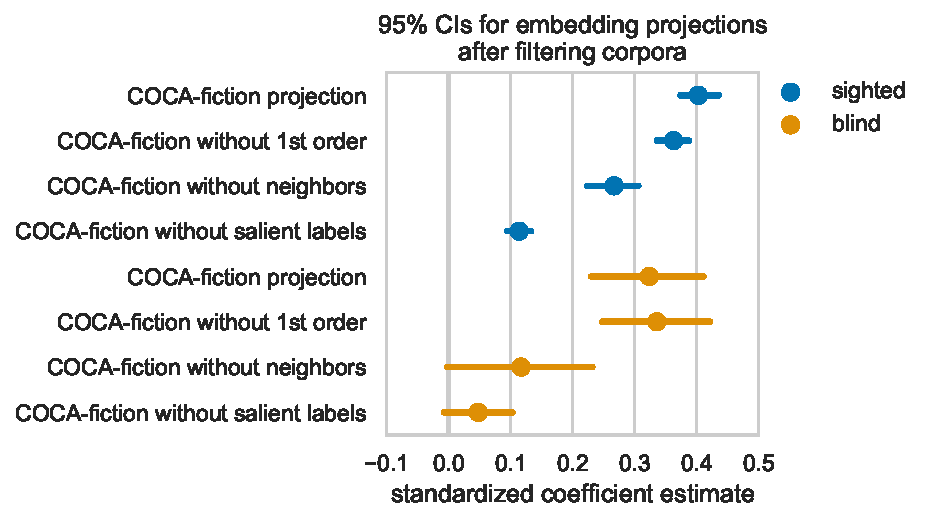
\includegraphics[width=\columnwidth]{figures/corpus_modification_forest_new.pdf}}
\caption{Estimated effects of word embedding projections in predicting blind and sighted participants' color-adjective association ratings.}
\label{corpus_modification}
\end{center}
\end{figure}

\section{Discussion}
That removing first-order co-occurrences had no measurable effect is perhaps not surprising: Word embedding models, specifically the skipgram models used here, are trained to predict the context a word occurs in. Strict first-order co-occurrence therefore does little to drive embedding similarity.

That instead removing participant-generated labels for color-adjective pairs is so effective in removing color-adjective association information from the embedding projections is striking, since the number of labels generated by at least two participants (the threshold for inclusion in our corpus filtering procedure) was only 242, on average less than one label per color-adjective pair. Furthermore, the positive correlation between name agreement (for the color-adjective pair labels) and association rating variability means that for color-adjective pairs with more salient labels, variability in ratings goes up, rather than down. This suggests that participant ratings are perhaps not directly mediated by availability of a salient label for a given color-adjective pair. Future work will explore whether the participant-generated labels also satisfy the second-order co-occurrence hypothesis, or if the semantic structures that underpin color-adjective associations arise from still higher-order co-occurrence patterns.

\begin{figure}[ht!]
\begin{center}
\fbox{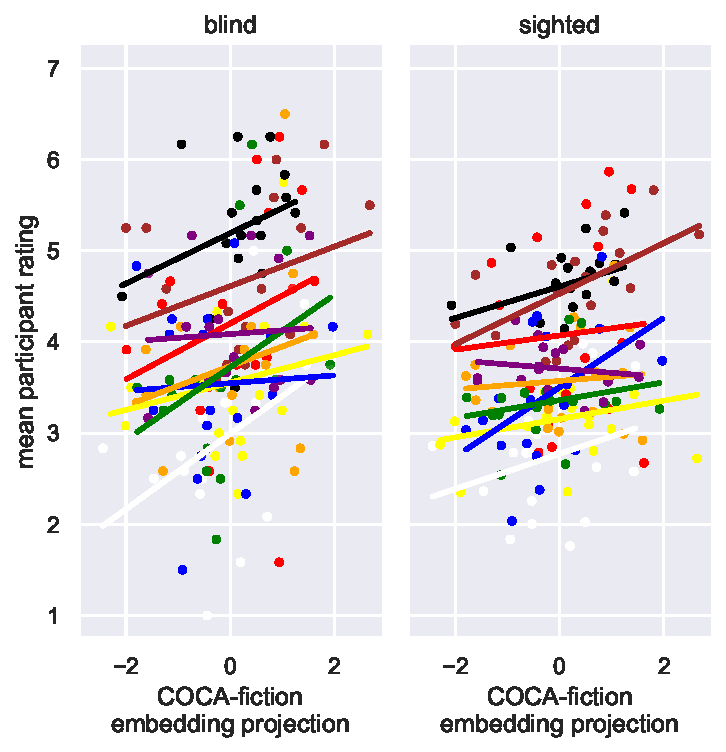
\includegraphics[width=\columnwidth]{figures/scatter_color.pdf}}
\caption{Mean participant rating versus embedding projection for each color-adjective association. Trendlines show positive relation between participants ratings and embedding projections across dimension for the majority of colors.}
\label{scatter_color}
\end{center}
\end{figure}

\section{General discussion}
\citeA{saysani2021seeing} demonstrated that blind people have color-adjective associations that are similar to those of sighted people. This is surprising in that many such associations would seem to require direct visual experience. \citeauthor{saysani2021seeing} surmised that blind people are likely learning about color-adjective relationships through language. Here, we show for the first time that the color-adjective associations captured in semantic differential tasks are present in the statistics of English. They are recoverable from a variety of corpora, but are best represented in a fiction corpus (see Figure \ref{scatter_color} for an illustration of both the relationship between ratings and embedding projections, and the similarity of this relationship across sighted and blind participants). 

In the subsequent studies, we examined whether people who report reading more fiction and/or have more print exposure in general show color-adjective associations that are more similar to those recoverable from the fiction corpus. No clear differences were found between people with different levels of print exposure or differences in self-reported fiction reading. 

We next examined \emph{where} in language these associations come from by altering the training corpus in an effort to remove likely linguistic sources of color-adjective associations. Removing first-order co-occurrences such as sentences containing colors and adjectives did nothing to disrupt the learned associations. On the other hand, removing sentences containing words that people think of when presented with color-adjective pairs sharply decreased the learned associations. These findings suggest that color-adjective associations in word embeddings are mediated by co-occurrence with salient words and that blind people are able to use this type of distributional semantic information to acquire color-adjective associations.

\section{Acknowledgments}
We would like to thank Armin Saysani and Michael and Paul Corballis for making available the raw data we reanalyzed in Experiment 1.

This research was supported by NSF BCS grant 2020969, awarded to Gary Lupyan.

\section{}
Data, code, and links to word embeddings are available at: \url{https://github.com/jvparidon/color-semantics/}

\bibliographystyle{apacite}

\setlength{\bibleftmargin}{.125in}
\setlength{\bibindent}{-\bibleftmargin}

\bibliography{color_semantics}


\end{document}
